\section{Relevant, extremal, and predecessor occurrences in a non-terminal}
\label{indexgapped:sec:occurrences}
In this section, we present a data structure that allows various efficient queries, which we will need to prove Theorem~\ref{thm:close_co_occurrences}.
We also show how it can be leveraged for an index in the simpler case of consecutive occurrences $(a = 0, b = N)$. 
Recall that the text $S$ is a string of length $N$ represented by an SLP $G$ of size $g$. By applying Lemma~\ref{lm:locally_consistent}, we transform $G$ into an RLSLP $G'$ of size $g' = O(g \log N)$ and depth $h = O(\log N)$ representing $S$, which we fix from now on. We start by showing that $G'$ can be processed in small space to allow multiple efficient queries:

\begin{restatable}{theorem}{occurrences}\label{th:occurrences}
There is a $O(g^2\log^4 N)$-space data structure for $G'$ that given a pattern $P$ of length $m$ can preprocess it in $O(m \log N + \log^2 N)$ time to support the following queries for a given non-terminal $A$ of $G'$:
\begin{enumerate}
\item Report the sorted set of relevant occurrences of $P$ in $\str{A}$ in $O(\log N)$ time;
\item Decide whether there is an occurrence of $P$ in $\str{A}$ in $O(\log N \log \log N)$ time;
\item Report the leftmost and the rightmost occurrences of $P$ in $\str{A}$, $\str{\head(A)}$, and $\str{\tail(A)}$ in $O(\log^2 N \log \log N)$ time;
\item Given a position $p$, find the rightmost (leftmost) occurrence $q \le p$ ($q \ge p$) of $P$ in $\str{A}$ in $O(\log^3 N \log \log N)$ time (predecessor/successor). 
\end{enumerate}
\end{restatable}
%
\noindent Before we proceed to the proof, let us derive a data structure to report all consecutive occurrences (co-occurrences) of a given pair of patterns.

\begin{corollary}\label{cor:all}
For an SLP of size $g$ representing a string $S$ of length $N$, there is an $O(g^2\log^4 N)$-space data structure that supports the following queries: given two patterns $P_1, P_2$ both of length $O(m)$, report all $\occ$ co-occurrences of $P_1$ and $P_2$ in $S$. The query time is $O(m\log N + (1+\occ) \cdot \log^3 N \log \log N)$. 
\end{corollary}
\begin{proof}
We exploit the data structure of Theorem~\ref{th:occurrences} for $G'$. To report all co-occurrences of $P_1,P_2$ in $S$, we preprocess $P_1,P_2$ in $O(m  \log N + \log^2 N)$ time and then proceed as follows. Suppose that we want to find the leftmost co-occurrence of $P_1$ and $P_2$ in the string $S[i\dots]$, where at the beginning $i=0$. We find the leftmost occurrence $q'_1$ of $P_1$ with $q'_1\geq i$ (if it exists) by a successor query on the initial symbol of $G'$ (the expansion of which is the entire string~$S$). Then we find the leftmost occurrence $q_2$ of $P_2$ with $q_2\geq q'_1$ (if it exists) by a successor query and the rightmost occurrence $q_1$ of $P_1$ with $q_1\leq q_2$ by a predecessor query. If either $q'_1$ or $q_2$ do not exist, then there are no more co-occurrences in $S[i\dots]$. Otherwise, clearly, $(q_1,q_2)$ is a co-occurrence, and there can be no other co-occurrences starting in $S[i\dots q_2]$. In this case, we return $(q_1,q_2)$ and set $i=q_2+1$. The running time of the retrieval phase is $O(\log^{3}N\log\log N\cdot (\occ+1))$, since we use at most three successor/predecessor queries to either output a new co-occurrence or decide that there are no more co-occurrences.
\end{proof}

\subsection{Proof of Theorem~\ref{th:occurrences}}
The data structure consists of two compact tries \Tpre\ and \Tsuf\ defined as follows. For each non-terminal $A$, we store $\rev{\str{\head(A)}}$ in \Tpre\ and $\str{\tail(A)}$ in  \Tsuf. We augment \Tpre\ and \Tsuf\ by computing their heavy path decomposition: 

\begin{definition}
The \emph{heavy path} of a trie $T$ is the path that starts at the root of $T$ and at each node $v$ on the path branches to the child with the largest number of leaves in its subtree (\emph{heavy} child), with ties broken arbitrarily. The heavy path decomposition is a set of disjoint paths defined recursively, namely it is defined to be a union of the singleton set containing the heavy path of $T$ and the heavy path decompositions of the subtrees of $T$ that hang off the heavy path. 
\end{definition}

For each non-terminal $A$ of $G'$, a heavy path $h_{pre}$ in \Tpre, and a heavy path $h_{suf}$ in \Tsuf, we construct a multiset of points $\Pset(A,h_{pre},h_{suf})$. For every non-terminal $A'$ and nodes $u \in h_{pre}$, $v \in h_{suf}$ the multiset contains a point $(|\lab(u)|, |\lab(v)|)$ iff $A', u, v$ satisfy the following properties:
\begin{enumerate}
\item $A$ is an ancestor of $A'$;
\item  \label{prop:leaves-below} $I(u)$ contains $\rev{\str{\head(A')}} $ and $I(v)$ contains $\str{\tail(A')} $. 
\item $u,v$ are the lowest nodes in $h_{pre}, h_{suf}$, respectively, satisfying Property~\ref{prop:leaves-below}.
\end{enumerate}
(See Fig.~\ref{fig:occurrences}.) The set 
$P(A,h_{pre},h_{suf})$ is stored in a two-sided 2D orthogonal range emptiness data structure~\cite{Lewenstein13,journals/talg/Chan13} which occupies  $O(|\Pset(A,h_{pre},h_{suf})|)$ space. 
 Given a 2D range of the form $[\alpha,\infty]\times[\beta,\infty]$, it allows to decide whether the range contains a point in $\Pset(A,h_{pre},h_{suf})$ in $O(\log\log N)$ time.
 

\begin{figure}
\centering
\captionsetup[subfigure]{justification=centering}
\begin{subfigure}[b]{0.4\textwidth}
\centering
%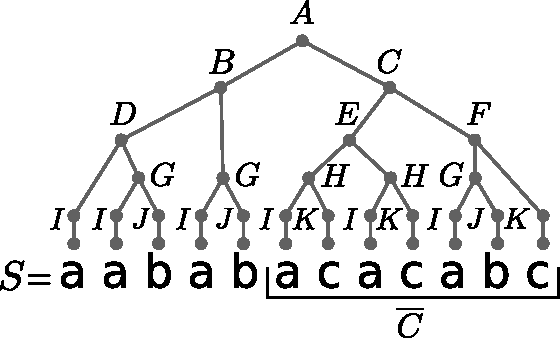
\includegraphics[width=\textwidth]{Part_One/index_gapped/figures/ex_parse_tree.pdf}
\caption{Parse tree of $G'$.}
\end{subfigure}
\hfill
\begin{subfigure}[b]{0.58\textwidth}
\centering
%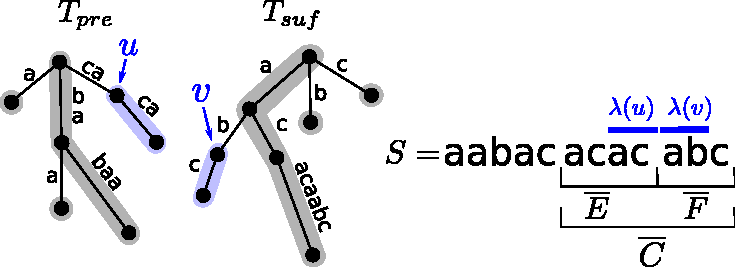
\includegraphics[width=\textwidth]{Part_One/index_gapped/figures/ex_Tpre_Tsuf.pdf}
\caption{Searching for \texttt{cab} with a split $s=1$.}
\end{subfigure}
\caption{A string $S=\mathrm{aababacacabc}$ is generated by an SLP $G'$. Nodes $u$ and $v$ are the loci of \texttt{c} and \texttt{ab} in \Tpre\  and \Tsuf\, respectively. The heavy paths $h_{pre}$ in \Tpre\ and $h_{suf}$ in \Tsuf\ are shown in blue. We have $(2,2) \in \Pset(A,h_{pre},h_{suf})$ corresponding to $C,u,v$.}
\label{fig:occurrences}
\end{figure}

\begin{claim}\label{claim:space-all}
The data structure occupies $O(g^2 \log^4 N)$ space.
\end{claim}
\begin{proof}
Each non-terminal $A'$ has at most $g'$ distinct ancestors and each root-to-leaf path in \Tpre\ or \Tsuf\ crosses $O(\log g')$ heavy paths (as each time we switch heavy paths, the number of leaves in the subtree of the current node decreases by at least a factor of two). As a corollary, each non-terminal creates $O(g' \log^2 g') = O(g \log^3 N)$ points across all orthogonal range emptiness data structures. 
\end{proof}


When we receive a pattern $P$, we compute $\splits(G',P)$ via Lemma~\ref{lm:locally_consistent} in $O(m \log N)$ time or provide a certificate that $P$ does not occur in $S$, in which case there are no occurrences of $P$ in the expansions of the non-terminals of $G'$. Recall that $|\splits(G',P)| \in O(\log N)$. We then sort $\splits(G',P)$ in $O(\log^2 N)$ time (a technicality which will allow us reporting relevant occurrences sorted without time overhead). Finally, we compute, for each $s \in \splits(G', P)$, the interval of strings in \Tpre\ prefixed by $\rev{P[\dots s]}$ (which is the interval $I(u)$ for the locus $u$ of $\rev{P[\dots s]}$ in \Tpre) and the interval of strings in \Tsuf\ prefixed by $P(s \dots ]$ (which is the interval $I(u)$ for the locus $u$ of $P(s \dots]$ in \Tsuf). By Lemma~\ref{lm:tries}, with $\tau=|\splits(G',P)|=O(\log N)$ and $h=O(\log N)$, this step takes $O(m+\log^2 N)$ time.

Reporting relevant occurrences is easy: by definition, each relevant occurrence $q$ of $P$ in $\str{A}$ is equal to $|\str{\head(A)}|-s$ for some  $s \in \splits(G',P)$ such that $\rev{P[\dots s]}$ is a prefix of $\rev{\str{\head(A)}}$ and $P(s\dots]$ is a prefix of $\str{\tail(A)}$. As we already know the intervals of the strings in \Tsuf\ and \Tpre\ starting with $\rev{P[\dots s]}$ and $P(s\dots]$, respectively, both conditions can be checked in constant time per split, or in $O(|\splits(G',P)|) = O(\log N)$ time overall. Note that since $\splits(G',P)$ are sorted, the relevant occurrences are reported sorted as well. 

We now explain how to answer emptiness queries on a non-terminal:
\begin{claim}\label{claim:emptiness}
Let $A$ be a non-terminal labeling a node in the parse tree of $G'$. We can decide whether $\str{A}$ contains an occurrence of $P$ in $O(\log N\log \log N)$ time. 
\end{claim} 
\begin{proof}
Below we show that $P$ occurs in $\str{A}$ iff there exists a split $s \in \splits(G',P)$ such that for $u$ being the locus of $\rev{P[\dots s]}$ in \Tpre\ and $v$ the locus of $P(s \dots]$ in \Tsuf , for $h_{pre}$ the heavy path containing $u$ in \Tpre and $h_{suf}$ the heavy path containing $v$ in \Tsuf , the rectangle $[|\lab(u)|,+\infty] \times [|\lab(v)|,+\infty]$ contains a point from $\Pset(A,h_{pre},h_{suf})$. Before we proceed to the proof, observe that by the bound on $|\splits(G',P)|$ this allows us to decide whether $P$ occurs in $\str{A}$ in $O(\log N)$ range emptiness queries, which results in $O(\log N\log \log N)$ query time. 

Assume that $[|\lab(u)|,+\infty] \times [|\lab(v)|,+\infty]$ contains a point $(x,y) \in \Pset(A,h_{pre},h_{suf})$ corresponding to a non-terminal $A'$. By construction, $A$ is an ancestor of $A'$, the subtree of $u$ contains a leaf corresponding to $\rev{\str{\head(A')}}$ and the subtree of $v$ contains a leaf corresponding to $\str{\tail(A')}$. Consequently, $\str{A'}$ contains an occurrence of $P$, which implies that $\str{A}$ contains an occurrence of $P$. 
%
To show the reverse direction, let $\ell = \off(u)+1$ and $r = \off(u)+|\str{A}|$, i.e. $S[\ell \dots r] = \str{A}$. The string $\str{A}$ contains an occurrence $\str{A}[q \ldots q+|P|)$ of $P$ iff $S[\ell+q \ldots \ell+q+|P|)$ is an occurrence of $P$ in $S$. From Claim~\ref{claim:primary_occurrence} it follows that if $w$ is the lowest node in the parse tree of $G'$ that contains leaves $S[\ell+q], \dots, S[\ell+q+|P|-1]$ in its subtree and $A'$ is its label, then there exists a split $s \in \splits(G',P)$ such that $\rev{P[\dots s]}$ is a prefix of $\rev{\str{\head(A')}}$ and $P(s\dots ]$ of $\str{\tail(A')}$. By definition of $u$ and $v$, the leaf of \Tpre\ labeled with $\rev{\str{\head(A')}}$ belongs to $I(u)$ and the leaf of \Tsuf\ labeled with $\str{\tail(A')}$ belongs to $I(v)$. Let $h_{pre}$ ($h_{suf}$) be the heavy path in \Tpre (\Tsuf) containing $u$ ($v$) and $(x,y)$ be the point in $\Pset(A,h_{pre},h_{suf})$ created for $A'$. As $|\lab(u)| \le x$ and $|\lab(v)| \le y$, the rectangle $[|\lab(u)|,+\infty] \times [|\lab(v)|,+\infty]$ is not empty.  
\end{proof}

It remains to explain how to retrieve the leftmost/rightmost occurrences in a non-terminal, as well as to answer predecessor/successor queries. The main idea for all four types of queries is to start at any node of the parse tree of $G'$ labeled by $A$ and recurse down via emptiness queries and case inspection. Since the length of the expansion decreases each time we recurse from a non-terminal to its child and the height of $G'$ is $h = O(\log N)$, this allows to achieve the desired query time. 
%We provide full details in Appendix~\ref{app:occurrences}. %\qed


\begin{claim}\label{claim:leftmost_rightmost}
Given a non-terminal $A$ of $G'$, we can find the leftmost and the rightmost occurrences of $P$ in $\str{A}$ and as a corollary in $\str{\head(A)}$ and $\str{\tail(A)}$ in $O(\log^{2} N\log\log N)$ time.  % h splits \log^{\eps} N
\end{claim}
\begin{proof}
We explain how to find the leftmost occurrence of $P$ in $\str{A}$, the rightmost one can be found analogously. We first check whether $\str{A}$ contains an occurrence of $P$ via Claim~\ref{claim:emptiness} in $O(\log N\log \log N)$ time. If it does not, we can stop immediately. Below we assume that there is an occurrence of $P$ in  $\str{A}$. Next, we check whether $\str{\head(A)}$ contains an occurrence of $P$ via Claim~\ref{claim:emptiness} in $O(\log N\log \log N)$ time. If it does, the leftmost occurrence of $P$ in $\str{A}$ is the leftmost occurrence of $P$ in $\str{\head(A)}$ and we can find it by recursing on $\head(A)$. If $\str{\head(A)}$ does not contain an occurrence of $P$, but $\str{A}$ contains relevant occurrences of $P$, then the leftmost occurrence of $P$ in $\str{A}$ is the leftmost relevant occurrence of $P$ in $\str{A}$ and we can find it in $O(|\splits(G',P)|) = O(\log N)$ time. Finally, if $P$ neither occurs in $\str{\head(A)}$ nor has relevant occurrences in $\str{A}$, then the leftmost occurrence of $P$ in $\str{A}$ is the leftmost occurrence of $P$ in $\str{\tail(A)}$. If $\tail(A)$ is a non-terminal $C$, we recurse on $C$ to find it. If $\tail(A)=B^{r-1}$ for a non-terminal $B$, $\str{\tail(A)}$ cannot contain an occurrence of $P$ because $\str{B}$ does not contain $P$ and there are no relevant occurrences in $A$. We recurse down at most $h = O(\log N)$ levels, and spend $O(\log N\log \log N)$ time per level. The claim follows.
\end{proof}

\begin{lemma}\label{lm:predecessor}
Let $A$ be a non-terminal of $G'$. For any position $p$, we can find the rightmost occurrence $q \le p$ of $P$ in $\str{A}$ and the leftmost occurrence $q'\geq p$ of $P$ in $\str{A}$ in $O(\log^{3} N\log \log N)$ time.  
\end{lemma}
\begin{proof}
First we describe how to locate $q$. Consider a node $u$ of the parse tree of $G'$ labeled by $A$. The algorithm starts at $u$ and recurses down. Let $A'$ be the label of the current node. It computes the leftmost and rightmost occurrences in $\str{A'}$, $\str{\head(A')}$ and $\str{\tail(A')}$ as well as all relevant occurrences via Claim \ref{claim:leftmost_rightmost}. If the leftmost occurrence of $P$ in $\str{A'}$ is larger than $p$, the search result is empty. Otherwise, consider two cases. 

\begin{enumerate}
\item $A'$ is associated with a rule $A' \rightarrow B'C'$, i.e. $\head(A') = B'$, $\tail(A') = C'$. 
\begin{enumerate}
\item If $p \le |\str{B'}|$, recurse on $B'$. 
\item Assume now that $p > |\str{B'}|$. If the leftmost  occurrence of $P$ in $\str{C'}$ is smaller than $p$, recurse on $C'$. Otherwise, return the rightmost relevant occurrence of $P$ in $\str{A'}$ if it exists else the rightmost occurrence of $P$ in $\str{B'}$. 
\end{enumerate}
\item $A'$ is associated with a rule $A \rightarrow (B')^r$, i.e. $\head(A') = B'$, $\tail(A') = (B')^{r-1}$.  Let an integer $k$ be such that $(k-1) \cdot |\str{B'}|+1 \le p \le k \cdot |\str{B'}|$. The desired occurrence of $P$ is the rightmost one of the following ones:
\begin{enumerate}
    \item The rightmost occurrence $q \le p$ of $P$ which crosses the border between two copies of $\str{B'}$. To compute $q$, we compute all relevant occurrences of $P$ in $\str{A'}$ and then shift each of them by the maximal possible shift $r' \cdot |\str{B'}|$, where $r'$ is an integer, which guarantees that it starts before $p$ and ends before $|\str{A'}|$ and take the rightmost of the computed occurrences to obtain $q$.
    \item The rightmost occurrence $q$ of $P$ such that for some integer $k'$, we have $(k'-1) \cdot |\str{B'}| \le q \le q+|P|-1 \le k' \cdot |\str{B'}|$ (i.e. the occurrence fully belongs to some copy of $\str{B'}$). In this case, $q$ is either the rightmost occurrence of $P$ in the $(k-1)$-th copy of $\str{B'}$, or the rightmost occurrence of $P$ in the $k$-th copy of $\str{B'}$ that is smaller than $p$. In the second case, we compute $q$ by recursing on $B'$.
    \end{enumerate}
\end{enumerate}
    We recurse down at most $h$ levels. On each level we spend $O(\log^{2} N\log\log N)$ time to compute the leftmost, the rightmost, and relevant occurrences and respective shifts for a constant number of non-terminals via Claim~\ref{claim:leftmost_rightmost}. Therefore, in total we spend $O(h \cdot \log^{2} N\log\log N) = O(\log^{3} N\log\log N)$ time. 
    
    
Locating $q'$ is very similar and differs only in small technicalities. The algorithm starts at the node $u$ and recurses down. Let $A'$ be the label of the current node. We compute the leftmost and rightmost occurrences in $\str{A'}$, $\str{\head(A')}$ and $\str{\tail(A')}$ as well as all relevant occurrences via Claim \ref{claim:leftmost_rightmost}. If the rightmost occurrence of $P$ in $\str{A'}$ is smaller than $p$, the search result is empty. Otherwise, consider two cases. 

\begin{enumerate}
\item $A'$ is associated with a rule $A' \rightarrow B'C'$, i.e. $\head(A') = B'$, $\tail(A') = C'$. 
\begin{enumerate}
\item If $p > |\str{B'}|$, recurse on $C'$. 
\item Assume now that $p \leq |\str{B'}|$. If the rightmost  occurrence of $P$ in $\str{B'}$ is larger than $p$, recurse on $B'$. Otherwise, return the leftmost relevant occurrence $q$ satisfying $q\geq p$, if it exists, and otherwise the leftmost occurrence of $P$ in $\str{C'}$. %Otherwise, return the rightmost relevant occurrence of $P$ in $\str{A'}$ if it exists else the rightmost occurrence of $P$ in $\str{B'}$. 
\end{enumerate}
\item $A'$ is associated with a rule $A \rightarrow (B')^r$, i.e. $\head(A') = B'$, $\tail(A') = (B')^{r-1}$.  Let an integer $k$ be such that $(k-1) \cdot |\str{B'}|+1 \le p \le k \cdot |\str{B'}|$. The desired occurrence of $P$ is the leftmost one of the following ones:
\begin{enumerate}
    \item The leftmost occurrence $q' \geq p$ of $P$ which crosses the border between two copies of $\str{B'}$. To compute $q'$, we compute all relevant occurrences of $P$ in $\str{A'}$ and then shift each of them by the minimal possible shift $r' \cdot |\str{B'}|$, where $r'$ is an integer, which guarantees that it starts after $p$ and ends before $|\str{A'}|$ (if it exists) and take the leftmost of the computed occurrences to obtain $q$.
    \item The leftmost occurrence $q'$ of $P$ such that for some integer $k'$, we have $(k'-1) \cdot |\str{B'}| \le q' \le q'+|P|-1 \le k' \cdot |\str{B'}|$ (i.e. the occurrence fully belongs to some copy of $\str{B'}$). In this case, $q'$ is either the leftmost occurrence of $P$ in the $(k+1)$-st copy of $\str{B'}$, or the leftmost occurrence of $P$ in the $k$-th copy of $\str{B'}$ that is larger than $p$. In the second case, we compute $q'$ by recursing on $B'$.
    \end{enumerate}
\end{enumerate}
The time complexities are the same as for computing $q$.
\end{proof}

